\documentclass[UTF8, 11pt]{ctexbeamer}
\definecolor{links}{HTML}{2A1B81}
\hypersetup{colorlinks,linkcolor=,urlcolor=links}
\usetheme[hideothersubsections]{Goettingen}
\usecolortheme{seahorse}
\graphicspath{{figures/}{images/}}
\usepackage{ulem}

% 删除 figurename
\setbeamertemplate{caption}{\raggedright\insertcaption\par}
% 解决目录间距过宽的问题
\usepackage{etoolbox}
\makeatletter
\patchcmd{\beamer@sectionintoc}{\vskip1.5em}{\vskip0.5em}{}{}
\makeatother

\AtBeginSection[]{
    \begin{frame}{本节提纲}
    \small\tableofcontents[currentsection,hideothersubsections]
    \end{frame}
}

\title{60 分钟入门 GMT}
\author{田冬冬}
\date{2016年9月21日}
\institute{中国科学技术大学}

\begin{document}

% 标题页
\begin{frame}
\titlepage
\end{frame}

\begin{frame}[<+->]{标题党}
\sout{60 分钟入门 GMT}
\pause
\begin{itemize}
\item 不确定讲完需要多久
\item 不确定讲完之后你能不能入门
\item 确定的是听完之后你还是不会画图
\end{itemize}
\onslide<+->{别怕,我会交给你学习的思路。}
\end{frame}

\begin{frame}{提纲}
\small
\tableofcontents[hidesubsections]
\end{frame}

\section{简介}
\subsection{是什么}
\begin{frame}{是什么}
\begin{figure}
\includegraphics[width=5cm]{GMT_logo}
\end{figure}
\begin{itemize}
\item Generic Mapping Tools
\item 通用制图工具
\item 官方网站:\url{http://gmt.soest.hawaii.edu}
    \begin{itemize}
    \item 下载任意版本的安装包以及源码
    \item 查看任意版本的文档
    \item 提问以获得帮助
    \item 提交 BUG
    \end{itemize}
\end{itemize}
\end{frame}

\subsection{历史}
\begin{frame}{历史}
\begin{itemize}
\item 1988年:研究生 Paul Wessel 和 Walter H.F. Smith 开发了GMT的最原始版本GMT 1.0
\item 1991年8月10日,GMT 2.x发布
\item 1998年11月8日,GMT 3.x发布
\item 2005年10月1日,GMT 4.x发布;目前最新版本GMT 4.5.14发布于2015-11-01
\item 2013年11月5日,GMT 5.x发布;目前最新版本GMT 5.2.1发布于2015-11-12
\end{itemize}
\end{frame}

\begin{frame}{开发团队}
\centering
\begin{figure}
\includegraphics[width=\textwidth]{GMT5_Summit_2016.jpg}
\end{figure}
Joaquim Luis, Walter H.F. Smith, \\
Remko Scharroo, Florian Wobbe, and Paul Wessel
\end{frame}

\subsection{版本}
\begin{frame}[fragile]{GMT4 vs GMT5}
\begin{block}{版本号的概念}
\centering\verb|major.minor.patch <=> 5.2.1|
\begin{itemize}
\item 当有极大的更新,会增加主版本号 major
\item 当有较大的更新,比如程序接口发生变化,会更新次版本号 minor
\item 若更新主要是修复错误,则会增加 patch 的版本号
\end{itemize}
\end{block}\pause
\begin{block}{GMT版本}
\begin{itemize}
\item GMT 5.x.x 和 GMT 4.x.x 差异很大,两个版本的语法不完全兼容
\item GMT 5.2.x 和 GMT 5.1.x 部分命令的语法和用法可能有一点区别
\item GMT 5.2.1 在 GMT 5.2.0 基础上修复了一些BUG
\end{itemize}
\end{block}
\end{frame}

\subsection{用途}
\begin{frame}{用途}
\begin{block}{绘图}
\begin{itemize}
\item 直角坐标系:线性坐标、对数坐标、指数坐标
\item 日期时间坐标
\item 极坐标系
\item 地图投影:30多种投影方式
\item 3D立体图
\end{itemize}
\end{block}
\begin{block}{数据处理}
\begin{itemize}
\item 数据滤波
\item 多项式拟合
\item 网格插值
\item ...
\end{itemize}
\end{block}
\end{frame}
\begin{frame}{示例: 线性坐标}
\includegraphics[width=\textwidth]{GMT_JX_linear}
\end{frame}
\begin{frame}{示例: 对数坐标}
\includegraphics[width=\textwidth]{GMT_JX_log}
\end{frame}
\begin{frame}{示例: 指数坐标}
\includegraphics[width=\textwidth]{GMT_JX_pow}
\end{frame}
\begin{frame}{示例: 日期时间坐标}
\includegraphics[width=\textwidth]{GMT_JX_calendar}
\end{frame}
\begin{frame}{示例: 极坐标}
\centering
\includegraphics[width=0.6\textwidth]{GMT_JP_polar}
\end{frame}
\begin{frame}{示例: 地理投影(全球)}
\centering
\includegraphics[width=0.9\textwidth]{GMT_geo_global}
\end{frame}
\begin{frame}{示例: 地理投影(区域)}
\centering
\includegraphics[width=0.8\textwidth]{GMT_geo_regional}
\end{frame}
\begin{frame}{示例: 立体图}
\centering
\includegraphics[width=0.6\textwidth]{GMT_3D}
\end{frame}

\begin{frame}{更多示例}
\begin{itemize}
\item GMT 官方示例:\url{http://gmt.soest.hawaii.edu/doc/latest/Gallery.html}
\item GMT 中文社区示例:\url{http://gmt-china.org}
\item SeisMan 博客示例:\url{https://seisman.info/tags/GMT/}
\end{itemize}
\end{frame}

\subsection{优缺点}
\begin{frame}{优缺点}
\begin{block}{优点}
\begin{itemize}
\item 开源免费,无版权问题
\item 跨平台:Linux、Windows、Mac等
\item 模块化
\item 命令行:可以精确控制所有细节,可以批量绘图
\item 输出矢量图,任意缩放不失真,可直接用于投稿
\end{itemize}
\end{block}
\pause
\begin{block}{缺点}
\begin{itemize}
\item 无 GUI
\item 中文文档较少
\item 无法满足所有画图需求
\end{itemize}
\end{block}
\end{frame}

\section{安装}
\subsection{Windows下的安装}
\begin{frame}{Windows:下载}
\begin{center}
\begin{tabular}{ c | l | l }
\hline
& 64位 & 32 位 \\
\hline
GMT & \href{http://mirrors.ustc.edu.cn/gmt/bin/gmt-5.2.1-win64.exe}{gmt-5.2.1-win64.exe} & \href{http://mirrors.ustc.edu.cn/gmt/bin/gmt-5.2.1-win32.exe}{gmt-5.2.1-win32.exe} \\
\hline
ghostscript & \href{https://github.com/ArtifexSoftware/ghostpdl-downloads/releases/download/gs919/gs919w64.exe}{gs919w64.exe} & \href{https://github.com/ArtifexSoftware/ghostpdl-downloads/releases/download/gs919/gs919w32.exe}{gs919w32.exe} \\
\hline
gsview & \href{http://pages.cs.wisc.edu/~ghost/gsview/download/gsv50w64.exe}{gsv50w64.exe} & \href{http://pages.cs.wisc.edu/~ghost/gsview/download/gsv50w32.exe}{gsv50w32.exe} \\
\hline
\end{tabular}
\end{center}

注意:GMT5 最新版不再支持 Windows XP!
\end{frame}
\begin{frame}{Windows:安装}
\centering
\includegraphics[width=0.9\textwidth]{GMT_win_install_1}
\end{frame}
\begin{frame}{Windows:安装}
\centering
\includegraphics[width=0.9\textwidth]{GMT_win_install_2}
\end{frame}
\begin{frame}{Windows:安装}
\centering
\includegraphics[width=0.9\textwidth]{GMT_win_install_3}
\end{frame}
\begin{frame}{Windows:安装}
``开始->附件->所有程序->命令提示符'' 以启动 cmd:\\
\centering
\includegraphics[width=0.7\textwidth]{GMT_win_install_4}
\end{frame}

\subsection{Mac下的安装}
\begin{frame}[fragile]{Mac: 安装}
\begin{enumerate}
\item 安装 Homebrew,见 \url{http://brew.sh/}
\item 安装 GMT
\begin{verbatim}
$ brew update && brew upgrade
$ brew tap homebrew/science
$ brew install gmt
\end{verbatim}
\item 使用 GMT
\begin{verbatim}
$ gmt --version
5.2.1
\end{verbatim}
\end{enumerate}
\end{frame}

\subsection{Linux下的安装}
\begin{frame}[fragile]{Linux: 安装}
见 \small{\url{http://docs.gmt-china.org/installation.html#linux}}
\begin{itemize}
\item 安装依赖包:netCDF、FFTW、cmake、glib2、ghostscript 等
\item 下载 GMT 源码包、全球海岸线数据GSHHG、全球数字图表DCW
\item 解压压缩文件
\item 修改配置文件 \verb|cmake/ConfigUser.cmake|
\item 编译及安装
\item 修改环境变量
\end{itemize}
\end{frame}

\subsection{初次运行}
\begin{frame}[fragile]{初次运行}
在 cmd 或终端中输入如下命令:\\
\verb|gmt pscoast -Rg -JH25c -Bafg -W1p > map.ps| \\[1cm]
\includegraphics[width=0.9\textwidth]{first_run}
\end{frame}

\section{基础知识}
\subsection{假如没有画图软件}
\begin{frame}{假如没有画图软件}
\begin{columns}
\column{0.68\linewidth}
假设回到没有计算机的时代:
\centering
\includegraphics[width=\textwidth]{handy_plot}
\pause
\column{0.3\linewidth}
我们需要:
\begin{itemize}
\item 画纸
\item 尺子
\item 画笔
\item 颜料
\item 文字
\item 数据
\end{itemize}
\end{columns}
\end{frame}

\subsection{设计理念}
\begin{frame}[fragile]{设计理念}
\begin{block}{命令的构成}
\verb|gmt + 模块 + 选项 + 参数 + 文件|
\end{block}\pause
\begin{block}{示例}
\scriptsize{\verb|gmt psxy input.dat -R0/20/0/20 -JM6i -W1p -B5 -B+t"First Figure" -P > map.ps|}
\end{block}
\begin{block}{说明}
\begin{itemize}
\item 从 GMT5开始,所有 GMT 命令都以 \verb|gmt| 开头,后面紧跟着模块名
\item 选项以 \verb|-| 开头,后接单个字符表示某个选项,字符后接选项的参数以及子选项
\item 子选项以 \verb|+| 开头,后接单个字符以及子选项的参数
\item 模块名、选项等均区分大小写
\item 各选项间以空格分隔,选项内部不能有空格
\item 选项内部的字符串若存在空格,应用单引号或双引号括起来
\end{itemize}
\end{block}
\end{frame}

\subsection{画纸}
\begin{frame}[fragile]{画纸: PostScript}
PostScript是一种用于描述矢量图形的页面描述语言。简单的说,用PostScript语言写成的文件就是PS格式的图片,一般文件后缀用 ps,简称为PS文件\pause
\begin{block}{PS 最小示例}
\small{
\begin{verbatim}
%! PS-Adobe-3.0
/Helvetica findfont 20 scalefont setfont
150 400 moveto
(PostScript is not that hard!) show

showpage
%%Trailer
%%EOF
\end{verbatim}
}
\end{block}
\end{frame}

\begin{frame}[fragile]{输出重定向}
GMT 中的画图命令会输出一堆 PostScript 语言的代码,需要将这些 PS 代码保存到 PS 文件中,
即输出重定向。

重定向符号的作用在于将命令的输出保存到文件中:
\begin{itemize}
\item \texttt{>}:若文件不存在,则新建文件;若文件已存在,则将原文件中的内容清空再将输出写入到文件中
\item \texttt{>>}:若文件不存在,则新建文件;若文件已存在,则将输出追加到文件的末尾
\end{itemize}

\begin{block}{示例}
\scriptsize{
\begin{verbatim}
gmt psxy -R0/100/0/10 -JX3i/1.5i -Bag -W1p -K sqrt.d > GMT_JX_linear.ps
gmt psxy -R -J -St0.1i -N -Gred -Wfaint -O sqrt.d10 >> GMT_JX_linear.ps
\end{verbatim}
}
\end{block}
\end{frame}

\subsection{尺子}
\begin{frame}{单位}
\begin{block}{长度单位}
\begin{itemize}
\item \texttt{p}:点(point),常用于比较小的量,比如线宽1.5p、文字大小15p
\item \texttt{c}:厘米(cm),常用于较大的量,比如底图宽度10c、圆半径0.5c
\item \texttt{i}:英寸(inch),用于较大的量,不推荐使用
\end{itemize}
1 inch = 2.54 cm = 72 point
\end{block}

\begin{block}{距离单位}
\begin{itemize}
\item d:弧度(degree of arc)
\item m:弧分(minute of arc)
\item s:弧秒(second of arc)
\item k:千米(kilometer)
\item e:米(meter);默认值
\end{itemize}
\end{block}
\end{frame}

\subsection{颜料}
\begin{frame}[fragile]{颜色:颜色名}
GMT 支持663种颜色名:
\begin{itemize}
\item white、black、red、orange、yellow、green、cyan、blue、magenta、gray、brown
\item light前缀:lightred、lightyellow 等
\item dark前缀:darkred、darkblue 等
\end{itemize}
颜色名不区分大小写。比如 lightblue、LIGHTBLUE、LightBlue 都是同一种颜色。
\end{frame}
\begin{frame}[fragile]{内置颜色名}
\includegraphics[width=\textwidth]{GMT_RGBchart}

\verb|${GMTHOME}/share/doc/pdf/GMT_RGBchart_a4.pdf|
\end{frame}

\begin{frame}[fragile]{颜色:RGB}
即三原色光模型,或又称RGB颜色模型,是一种加色模型,将红(Red )、绿(Green)、蓝(Blue)三原色的色光以不同的比例相加,以产生多种多样的色光。

格式:\verb|r/g/b|

取值范围:R、G、B 的取值范围是0到255内的整数

\begin{itemize}
\item 255/0/0: 红色
\item 0/255/0: 绿色
\item 0/0/255: 蓝色
\item 0/0/0: 黑色
\item 255/255/255: 白色
\end{itemize}
\end{frame}

\begin{frame}[fragile]{颜色:HSV}
格式:\verb|h-s-v|
\begin{itemize}
\item H:色相,是色彩的基本属性,就是平常所说的颜色名称,如红色、黄色等,取值范围为0到360。
\item S:饱和度,是指色彩的纯度,越高色彩越纯,低则逐渐变灰,取值范围为0到1。
\item V:明度,是色彩的亮度,取值范围为 0(暗)到1(亮)
\end{itemize}
示例:180-0-0、120-0.3-0.4
\end{frame}

\begin{frame}[fragile]{颜色:CMYK}
印刷四分色模式,是彩色印刷时采用的一种套色模式,利用色料的三原色混色原理,加上黑色油墨,共计四种颜色混合叠加,形成所谓“全彩印刷”。

格式:\verb|c/m/y/k| \\
\begin{itemize}
\item Cyan:青色,又称为天蓝色或是湛蓝
\item Magenta:品红色,又称为洋红色
\item Yellow:黄色
\item blacK:定位套版色(黑色)
\end{itemize}

取值范围:0到1 \\
示例:0/0/0/0,0.1/0.3/1/0.3
\end{frame}

\begin{frame}[fragile]{颜色:灰色}
\begin{itemize}
\item 用一个数值表示灰度即可,其取值范围为0到255。例如 0 表示黑色, 255 表示白色, 128 表示灰色。
\item 灰色本质上就是 R=G=B 的一种颜色。因而 128/128/128 代表灰度为 128
\item gray0, gray1 ... gray99, gray100
\end{itemize}
\end{frame}

\begin{frame}{透明}
\begin{itemize}
\item 每一种颜色都可以额外指定透明度
\item GMT中,可以通过在颜色后加上 @ 再加上透明度来得到不同程度的透明色
\item 透明度的取值范围是0到100,0表示不透明,100表示全透明
\end{itemize}

示例:red@25 、 30/25/128@60 。
\end{frame}

\begin{frame}{颜色小结}
\begin{itemize}
\item 颜色名: blue, lightred, darkyellow
\item RGB: 230/203/23, 130/45/78
\item HSV: 150-0.2-0.3, 350-0.1-0.1
\item CMYK: 0.2/0.3/0.4/0.5
\item 灰度: 0, 128, 255, gray0, gray128, gray255
\item 透明色: blue@20, 230/203/23@30, 350-0.1-0.1@60, 0.2/0.3/0.4/0.5@90
\end{itemize}
\end{frame}

\subsection{画笔}
\begin{frame}[fragile]{画笔}
格式:\verb|宽度,颜色,线型|
\begin{block}{宽度}
\begin{itemize}
\item 宽度值,比如1p、2.5p
\item 预定义宽度名:faint, thin, thick 等等
\end{itemize}
\end{block}
\end{frame}

\begin{frame}[fragile]{画笔}
格式:\verb|宽度,颜色,线型|
\begin{block}{线型}
\begin{itemize}
\item 预定义线型名:solid(实线)、dashed(虚线)、dotted(点线)
\item 简单符号:破折号 - 代表虚线、点号 . 代表点线
\item 组合符号:.-  ..-
\item 自定义线型:\verb|4_8_5_8:2|
\end{itemize}
\end{block}
\centering
\includegraphics[width=0.8\textwidth]{GMT_pens_examples}
\end{frame}

\subsection{文字}
\begin{frame}[fragile]{文字: 字号}
格式: \verb|size,fonttype,fill=pen|
\begin{block}{字号}
\begin{center}
\begin{tabular}{c|c|c|c}
\hline
字号 & p	  & 字号	& p  \\
\hline
初号 & 42	  & 小初	& 36 \\
一号 & 26	  & 小一	& 24 \\
二号 & 22	  & 小二	& 18 \\
三号 & 16	  & 小三	& 15 \\
四号 & 14	  & 小四	& 12 \\
五号 & 10.5 &	小五	& 9  \\
六号 & 7.5  &	小六	& 6.5\\
七号 & 5.5  &	八号	& 5  \\
\hline
\end{tabular}
\end{center}
\end{block}
\end{frame}

\begin{frame}[fragile]{文字: 字体}
格式: \verb|size,fonttype,fill=pen|
\begin{block}{字体}
可以用字体名,也可以用字体号
\begin{center}
\includegraphics[width=0.8\textwidth]{GMT_fonts}
\end{center}
\end{block}
\end{frame}

\begin{frame}[fragile]{文字: 填充与描边}
格式: \verb|size,fonttype,fill=pen| \\
\begin{block}{填充与描边}
\begin{center}
\includegraphics[width=0.8\textwidth]{GMT_text_examples}
\end{center}
\end{block}
\end{frame}

\subsection{数据}
\begin{frame}[fragile]{点/线数据}
\begin{columns}
\column{0.5\linewidth}
绘制一条线段:
\begin{verbatim}
0.2 0.5
0.4 0.6
1.2 1.0
2.3 3.4
\end{verbatim}
\column{0.5\linewidth}
绘制多段线段:
\begin{verbatim}
>
0.2 0.5
0.4 0.6
1.2 1.0
2.3 3.4
>
0.3 3.2
0.5 2.6
0.7 1.4
1.0 0.3
\end{verbatim}
\end{columns}
\end{frame}

\section{选项}
\subsection{标准选项}
\begin{frame}[fragile]{标准选项}
GMT 的每个模块都有众多选项,其中的某些选项是标准选项。标准选项在所有模块中具有完全相同的含义和语法。
\tiny
\begin{center}
\begin{tabular}{ll}
选项 & 说明 \\
\hline
-B & 定义底图边框和轴的刻度、标注、标签等属性 \\
-J & 选择地图投影方式或坐标变换 \\
-K & 省略PS文件尾以追加更多PS代码 \\
-O & 省略文件头以将PS代码追加到已有的文件中 \\
-P & 设置纸张方向为Portrait模式 \\
-R & 指定区域范围 \\
-U & 在图上绘制时间戳 \\
-V & 详细报告模式 \\
-X & 移动X方向上的绘图原点 \\
-Y & 移动Y方向上的绘图原点 \\
-a & 将非空间数据与某些列联系在一起 \\
-b & 控制二进制的输入或输出 \\
-c & 设置当前PS文件打印时的份数 \\
-d & 将输入或输出中的 nodata 替换成NaN \\
-f & 设置ASCII输入或输出的格式 \\
-g & 根据数据间断对数据进行分段 \\
-h & 跳过数据的文件头段记录 \\
-i & 选择输入列 \\
-n & 设置网格插值方式 \\
-o & 选择输出列 \\
-p & 控制3D视角图 \\
-r & 设置网格配准方式 \\
-s & 控制NaN记录的处理方式 \\
-t & 设置图层透明度 \\
-x & 设置并行的核数(仅限于支持并行的模块)\\
-: & 输入数据是 y/x 而不是 x/y \\
\end{tabular}
\end{center}
\end{frame}

\subsection{-R}
\begin{frame}[fragile]{-R: 数据范围}
语法:
\begin{itemize}
\item \verb|-R<xmin>/<xmax>/<ymin>/<ymax>|
\item \verb|-R<xlleft>/<ylleft>/<xuright>/<yuright>r|
\end{itemize}
\includegraphics[width=0.8\textwidth]{GMT_-R}\\
示例:\\
-R-90/-70/18/37、-R-90/20/-65/28r、\\
-R0/360/-90/90(-Rg)、-R-180/180/-90/90(-Rd)
\end{frame}

\subsection{-J}
\begin{frame}[fragile]{-J:投影方式}
语法:
\begin{itemize}
\item \verb|-J<小写字母>[<pars>/]<scale>|
\item \verb|-J<大写字母>[<pars>/]<width>|
\end{itemize}
示例:
\begin{itemize}
\item \verb|-JX10c/5c| 使用线性投影,底图的宽度是10厘米,高度为5厘米
\item \verb|-Jm1c| 表示使用墨卡托投影,地图上的1度距离投影到画布上为1厘米
\item \verb|-Jm1:10000000| 表示使用墨卡托投影,画布上的1 cm代表实际距离中的10000000 cm,即100 km
\item \verb|-JM15c| 也表示使用墨卡托投影,整个地图的宽度是15厘米,地图的高度由 -R 和 -J 自动
\end{itemize}
\end{frame}

\subsection{-B}
\begin{frame}[fragile]{-B: 底图边框}
\begin{block}{轴属性}
\small{\verb!-B[x|y]<intervals>[+l|L<label>][+p<prefix>][+u<unit>]!}\pause
\end{block}
\begin{block}{示例}
\centering
\small\verb!gmt psbasemap -R0/10/0/5 -JX10c/5c -Bx2 > GMT_B_example_1.ps! \\[0.5cm]
\includegraphics[width=0.75\textwidth]{GMT_B_example_1}
\end{block}
\end{frame}

\begin{frame}[fragile]{-B: 底图边框}
\begin{block}{轴属性}
\small{\verb!-B[x|y]<intervals>[+l|L<label>][+p<prefix>][+u<unit>]!}
\end{block}
\begin{block}{示例}
\centering
\small\verb!gmt psbasemap -R0/10/0/5 -JX10c/5c -Bxa2f1g0.5 > B2.ps! \\[0.5cm]
\includegraphics[width=0.75\textwidth]{GMT_B_example_2}
\end{block}
\end{frame}

\begin{frame}[fragile]{-B: 底图边框}
\begin{block}{轴属性}
\small{\verb!-B[x|y]<intervals>[+l|L<label>][+p<prefix>][+u<unit>]!}
\end{block}
\begin{block}{示例}
\centering
\small\begin{verbatim}
gmt psbasemap -R0/10/0/5 -JX10c/5c \
    -Bxa2f1g0.5+l"X axis" > B3.ps
\end{verbatim}
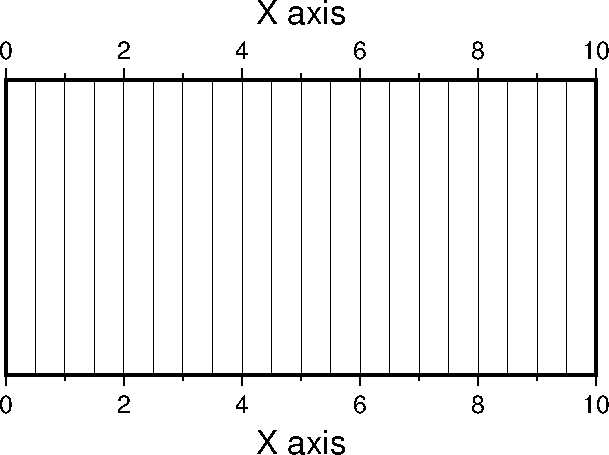
\includegraphics[width=0.6\textwidth]{GMT_B_example_3}
\end{block}
\end{frame}

\begin{frame}[fragile]{-B: 底图边框}
\begin{block}{轴属性}
\small{\verb!-B[x|y]<intervals>[+l|L<label>][+p<prefix>][+u<unit>]!}
\end{block}
\begin{block}{示例}
\centering
\small\begin{verbatim}
gmt psbasemap -R0/10/0/5 -JX10c/5c \
    -Bxa2f1g0.5+p'$' > B4.ps
\end{verbatim}
\includegraphics[width=0.6\textwidth]{GMT_B_example_4}
\end{block}
\end{frame}

\begin{frame}[fragile]{-B: 底图边框}
\begin{block}{轴属性}
\small{\verb!-B[x|y]<intervals>[+l|L<label>][+p<prefix>][+u<unit>]!}
\end{block}
\begin{block}{示例}
\centering
\small\begin{verbatim}
gmt psbasemap -R0/10/0/5 -JX10c/5c \
    -Bxa2f1g0.5+u'%' > B5.ps
\end{verbatim}
\includegraphics[width=0.6\textwidth]{GMT_B_example_5}
\end{block}
\end{frame}

\begin{frame}[fragile]{-B: 底图边框}
\begin{block}{轴属性}
\small{\verb!-B[x|y]<intervals>[+l|L<label>][+p<prefix>][+u<unit>]!}
\end{block}
\begin{block}{示例}
\centering
\small\begin{verbatim}
gmt psbasemap -R0/10/0/5 -JX10c/5c -Bx2+lX -By1+lY > B6.ps
\end{verbatim}
\includegraphics[width=0.6\textwidth]{GMT_B_example_6}
\end{block}
\end{frame}

\begin{frame}[fragile]{-B: 底图边框}
\begin{block}{边框属性}
\small{\verb!-B[<axes>][+g<fill>][+t<title]!}
\end{block}
\begin{itemize}
\item \verb|<axes>| 控制显示底图的哪几条边,以及如何显示
    \begin{itemize}
    \item 四条边分别用东西南北四个方向的首字母 E、W、S、N 表示
    \item 不出现该字母表示不绘制这条边
    \item 用大写字母表示绘制这条边,且该边有刻度、有标注
    \item 用小写字母表示绘制这条边,但该边有刻度、无标注
    \end{itemize}
\item \verb|+g<fill>| 设置底图的填充色
\item \verb|+t<title>| 设置图标题
\end{itemize}
\end{frame}

\begin{frame}[fragile]{-B: 底图边框}
\begin{block}{边框属性}
\small{\verb!-B[<axes>][+g<fill>][+t<title]!}
\end{block}
\begin{block}{示例}
\centering
\small\begin{verbatim}
gmt psbasemap -R0/10/0/5 -JX10c/5c -Bx2+lX -By1+lY -BWS > B7.ps
\end{verbatim}
\includegraphics[width=0.6\textwidth]{GMT_B_example_7}
\end{block}
\end{frame}

\begin{frame}[fragile]{-B: 底图边框}
\begin{block}{边框属性}
\small{\verb!-B[<axes>][+g<fill>][+t<title]!}
\end{block}
\begin{block}{示例}
\centering
\small\begin{verbatim}
gmt psbasemap -R0/10/0/5 -JX10c/5c -Bx2+lX -By1+lY -BWSen > B8.ps
\end{verbatim}
\includegraphics[width=0.6\textwidth]{GMT_B_example_8}
\end{block}
\end{frame}

\begin{frame}[fragile]{-B: 底图边框}
\begin{block}{边框属性}
\small{\verb!-B[<axes>][+g<fill>][+t<title]!}
\end{block}
\begin{block}{示例}
\centering
\small\begin{verbatim}
gmt psbasemap -R0/10/0/5 -JX10c/5c -Bx2+lX -By1+lY \
    -BWSen+glightblue+t'GMT is easy to learn' > B9.ps
\end{verbatim}
\includegraphics[width=0.6\textwidth]{GMT_B_example_9}
\end{block}
\end{frame}

\begin{frame}[fragile]{-B: 底图边框}
\begin{block}{小技巧}
\centering
\small\begin{verbatim}
gmt psbasemap -R0/10/0/5 -JX10c/5c -Bxafg -Byafg \
    -BWSen+glightblue+t'GMT is easy to learn' > B10.ps
\end{verbatim}
\includegraphics[width=0.6\textwidth]{GMT_B_example_10}
\end{block}
\end{frame}

\subsection{-P}
\begin{frame}{-P:纸张方向}
GMT中的纸张默认是Landscape(风景画)模式,使用-P选项则变成 Portrait(肖像)模式。
\centering
\includegraphics[width=\textwidth]{GMT_-P}
\end{frame}

\subsection{-V}
\begin{frame}[fragile]{-V: 进程报告}
\begin{itemize}
\item \verb|-Vq|:quiet;不输出任何错误和警告;
\item \verb|-Vn| :nomral;仅输出致命错误信息;即不使用 -V 选项时的默认值;
\item \verb|-Vc| :compatibility;输出兼容性相关的警告信息;
\item \verb|-Vv| 或 \verb|-V| :verbose;即输出错误、警告以及数据处理的基本信息;
\item \verb|-Vl| :long;详细的进程报告;
\item \verb|-Vd| :debug;包含了大量调试信息;
\end{itemize}
\end{frame}

\subsection{-U}
\begin{frame}[fragile]{-U: 时间戳}
语法: \verb!-U[<just>/<dx>/<dy>/][c|<label>]! \\

示例:\verb!-UBL/-1.5c/-1.5c/"This is a GMT logo"! \\[0.5cm]
\includegraphics[width=\textwidth]{GMT_-U}
\end{frame}

\subsection{-K和-O}
\begin{frame}[fragile]{-K 和-O:图层}
通常,一张图需要使用多个 GMT 绘图命令才能完成。每个绘图命令只完成了整张图的一个图层,
后面的命令生成的图层会叠加在前面的命令生成的图层之上。
\centering
\includegraphics[width=0.9\textwidth]{GMT_geo_global}
\begin{verbatim}
gmt xxx ... xxx -K > map.ps
gmt xxx ... xxx -K -O >> map.ps
gmt xxx ... ... -O >> map.ps
\end{verbatim}
\end{frame}
\begin{frame}[fragile]{-K 和-O:图层}
\includegraphics[width=\textwidth]{GMT_-OK}
\begin{verbatim}
gmt xxx ... xxx -K > map.ps
gmt xxx ... xxx -K -O >> map.ps
gmt xxx ... ... -O >> map.ps
\end{verbatim}
\end{frame}

\subsection{-X和-Y}
\begin{frame}[fragile]{-X和-Y:底图原点}
语法:\verb!-X[a|c|f|r][<xshift>[<u>]]!
\includegraphics[width=\textwidth]{GMT_-XY}
\end{frame}
\begin{frame}[fragile]{-X和-Y:底图原点}
语法:\verb!-X[a|c|f|r][<xshift>[<u>]]!
\begin{itemize}
\item -X2i 或 -Xr2i :在原底图原点的基础上沿X方向偏移2英寸得到新底图原点
\item -Xa5c :在原底图原点的基础上沿X方向偏移5厘米得到临时底图坐标,当前命令执行完成后,底图原点复原到原底图原点
\item -Xc3c :在纸张中心的基础上沿X方向偏移3厘米得到新底图原点
\item -Xf4c :在纸张左下角的基础上沿着X方向偏移4厘米得到新底图原点
\end{itemize}
\end{frame}

\section{配置文件}
\subsection{默认参数}
\begin{frame}[fragile]{默认参数}
\centering
\small\begin{verbatim}
gmt psbasemap -R0/10/0/5 -JX10c/5c -Bxafg -Byafg \
    -BWSen+glightblue+t'GMT is easy to learn' > B10.ps
\end{verbatim}
\includegraphics[width=0.6\textwidth]{GMT_B_example_10}

这些默认的属性由默认参数控制。默认参数保存在 gmt.conf 文件中。GMT 本身自带一个系统级别的 gmt.conf 文件,
同时,每个目录下也可以有自己的 gmt.conf 文件。GMT 命令在执行时会优先读取当前目录下的 gmt.conf 文件。
\end{frame}
\begin{frame}{默认参数}
\includegraphics[width=\textwidth]{GMT_Defaults_1}
\end{frame}
\begin{frame}{默认参数}
\includegraphics[width=\textwidth]{GMT_Defaults_2}
\end{frame}
\begin{frame}{默认参数}
\includegraphics[width=\textwidth]{GMT_Defaults_3}
\end{frame}
\subsection{修改默认参数}
\begin{frame}[fragile]{修改默认参数}
两种修改默认参数的方法:
\begin{itemize}
\item \verb|gmt gmtset FONT_TITLE 15p,8,red| 会在当前目录下生成 gmt.conf 文件,该命令的修改永久有效,除非 gmt.conf 文件被改回或被删除
\item \verb|gmt pscoast ... --FONT_TITLE=15p,8,red ... > map.ps| 仅对当前命令有效
\end{itemize}
\end{frame}

\section{常用命令}
\begin{frame}{GMT命令之绘图命令}
\begin{center}
\small
\begin{tabular}{ll}
\hline
命令 & 说明 \\
\hline
psbasemap & 绘制底图 \\
pscoast & 在地图上绘制海岸线、河流、国界线 \\
psxy & 在图上绘制线段、多边形和符号 \\
pstext & 在图上写文本 \\
psscale & 在图上绘制灰色或彩色色标 \\
psclip & 打开或关闭多边形裁剪路径 \\
psimage & 将图片或EPS文件放在地图上 \\
pslegend & 绘制图例 \\
pshistogram & 统计并绘制直方图 \\
psrose & 绘制极坐标下的直方图\\
psmeca & 在地图上绘制震源机制解 \\
pspolar & 在震源球上绘制台站极性 \\
psvelo & 在地图上绘制速度矢量、十字线、楔形图 \\
pscoupe & 绘制震源机制解的剖面图 \\
grdvector & 根据两个网格文件绘制矢量场 \\
grdimage & 在图上绘制网格数据 \\
gmtlogo & 在图上绘制GMT图形logo \\
\hline
\end{tabular}
\end{center}
\end{frame}

\begin{frame}{GMT命令之1D数据处理}
\begin{center}
\small
\begin{tabular}{ll}
\hline
命令 & 说明 \\
\hline
filter1d & 对1D表数据做时间域滤波 \\
gmtsimplify & 使用Douglas-Peucker算法对线段做简化 \\
gmtconnect & 将端点接近的线段连接起来 \\
sample1d & 对1D表数据进行重采样 \\
project & 将数据点投影到线或大圆路径上,生成测线,坐标转换 \\
\hline
\end{tabular}
\end{center}
\end{frame}

\begin{frame}{GMT命令之2D数据处理}
\begin{center}
\scriptsize
\begin{tabular}{ll}
\hline
命令 & 说明 \\
\hline
grdedit & 修改网格文件的头段或内容 \\
grdcut & 从一个网格文件中裁剪出一个子区域 \\
grdblend & 将多个部分重叠的网格文件合并成一个网格文件 \\
grdpaste & 将两个网格沿着其共同边界拼接成一个文件 \\
grdraster & 从二进制数据中提取子区域并保存为GMT网格文件 \\
grdclip & 对网格文件的Z值做裁剪 \\
grdlandmask & 根据海岸线数据创建陆地-海洋的mask网格文件 \\
grdtrend & 拟合网格的趋势面并计算残差 \\
grdsample & 对网格文件做重采样 \\
grdvolume & 计算网格数据中某个等值线所包围的表面积和体积 \\
grdproject & 对网格数据做地图变换和逆变换 \\
grdmask & 根据多边形数据或点数据创建mask网格文件 \\
grdconvert & 在不同的网格格式之间互相转换 \\
\hline
\end{tabular}
\end{center}
\end{frame}

\section{学习资源}
\subsection{学习资源}
\begin{frame}{学习资源}
\begin{itemize}
\item GMT官方文档: \scriptsize{\url{http://gmt.soest.hawaii.edu/doc/latest/index.html}}
\item GMT中文社区: \url{http://gmt-china.org}
\item GMT参考手册: \url{http://docs.gmt-china.org/}
\item GMT模块手册: \url{http://modules.gmt-china.org/}
\item GMT示例集: \url{http://examples.gmt-china.org/}
\item 地学GMT学习群:群号 218905582
\end{itemize}
\end{frame}

\subsection{如何学习 GMT}
\begin{frame}{如何学习 GMT}
\begin{itemize}
\item 根据自己所用的 GMT 版本看对应版本的文档
\item 如果有能力,尽量看官方英文版
\item 看《GMT 参考手册》,掌握其中提到的基础知识
\item 浏览一遍 GMT 的所有模块,对每个模块可以做什么要有印象
\item 根据绘图需求找到自己需要使用的模块,看模块的帮助文档
\item 看例子,多修改以查看不同参数的效果
\end{itemize}
\end{frame}

\section{中文社区}
\begin{frame}{为什么要建立中文社区}
\includegraphics[width=\textwidth]{GMT_china_homepage}
\end{frame}
\begin{frame}{社区做了哪些事}
\begin{itemize}
\item 翻译整理了中文手册:参考手册和模块手册
\item 建立社区网站
\item 国内下载镜像: \url{http://mirrors.ustc.edu.cn/gmt/}
\item GMT5 可用的 pssac
\item 组织培训及线下聚餐
\end{itemize}
\end{frame}

\begin{frame}{还需要做哪些事情}
\begin{itemize}
\item GMT 中文社区 logo
\item 完成尚未翻译整理的部分
\item 提交示例
\item 报告 BUG
\item 重新设计并维护网站
\item 其他...
\end{itemize}
\end{frame}

\begin{frame}
    \Large\centering Thank you!
\end{frame}
\end{document}
